\begin{boxE}
 \lr{
 \lstinputlisting[language=Python]{IR5/code/job_3.py}
 }   
\end{boxE}

\begin{figure}
    \centering
    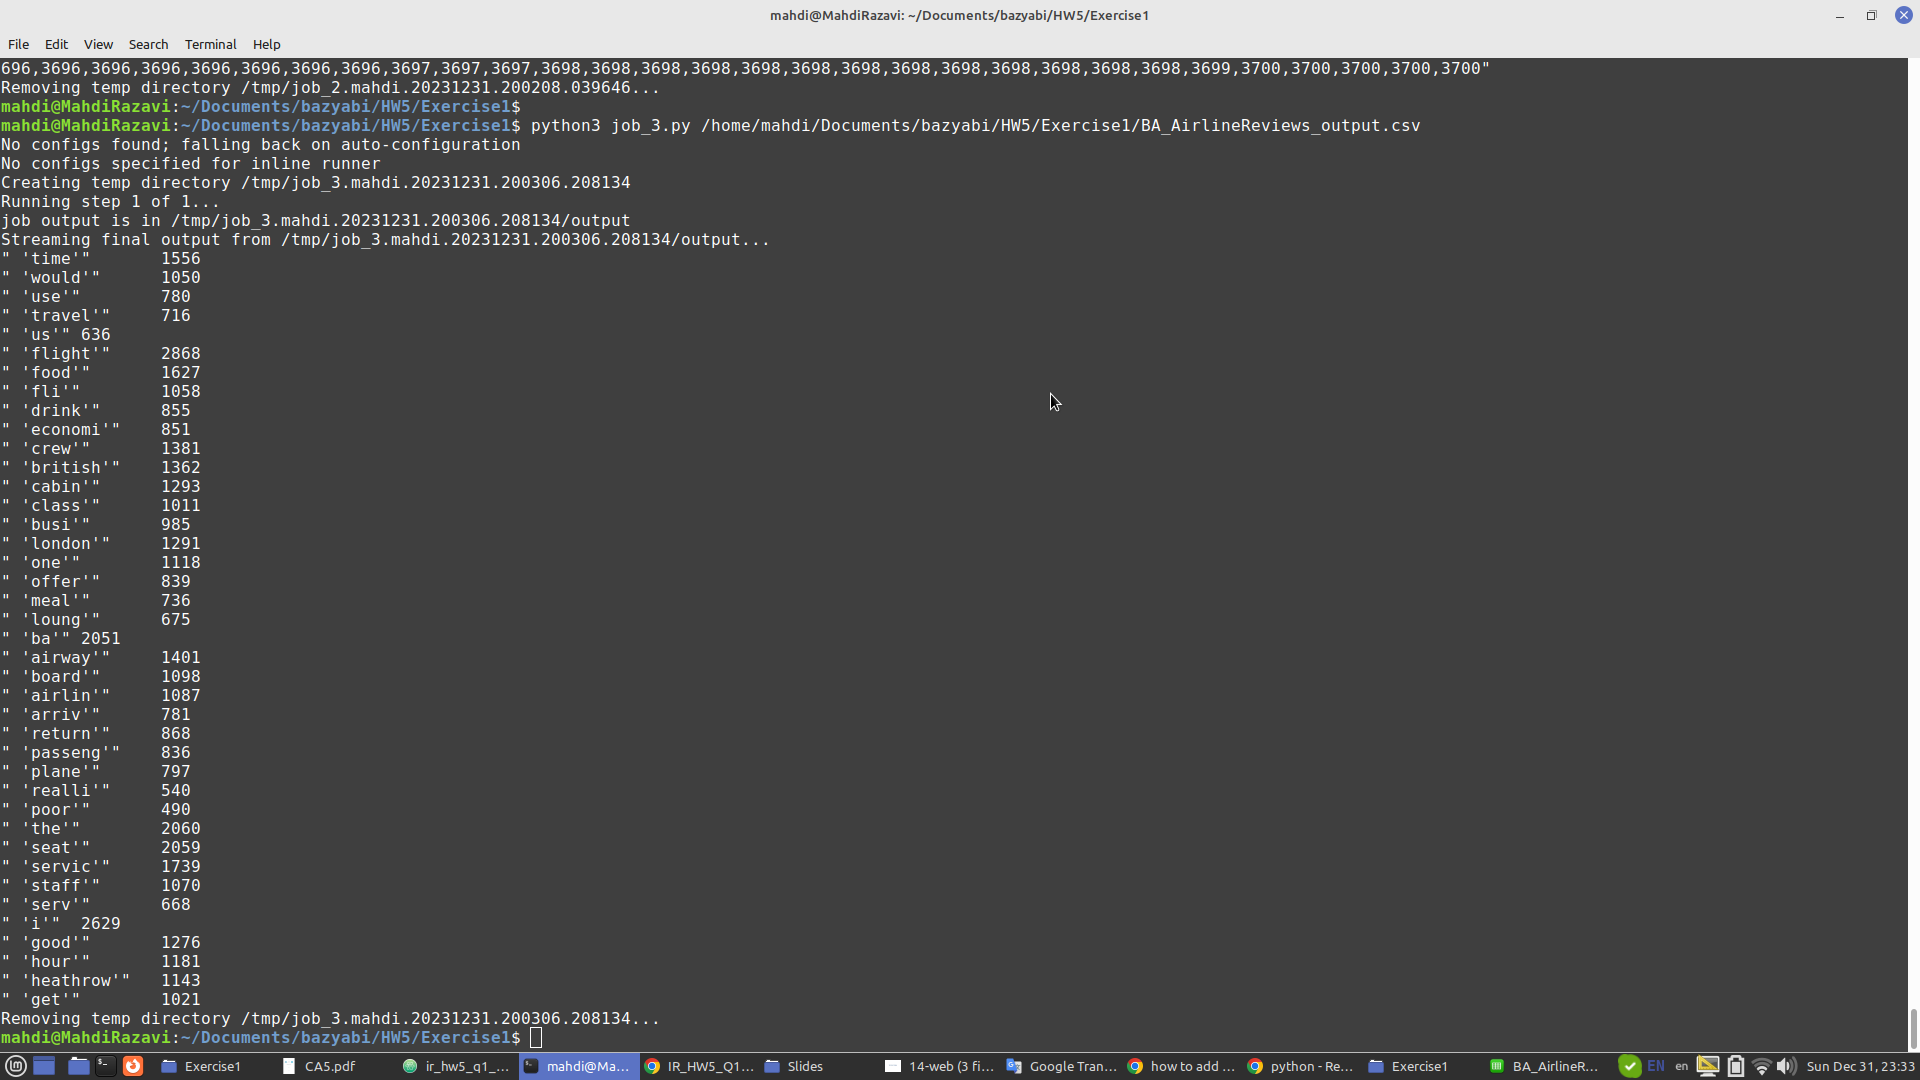
\includegraphics
    [width = 0.9\textwidth]
    {IR5/image/MapReduce3.png}
    \caption{
    کلماتی که در بیشترین بازخورد ظاهر شده‌اند.
    }
    \label{fig:enter-label}
\end{figure}

\begin{boxM}
    این تمرین بسیار شبیه به 
    \lr{job1}
    می‌باشد . 
    با این تفاوت که باید کلمات را بشماریم.

    ابتدا هر کلمه ظاهر شده در متن پیش‌پردازش شده‌مان را به عدد یک نظیر خواهیم کرد.
    سپس گام 
    \lr{Reducer}
    ما به ۳ تا زیرگام تقسیم خواهدشد.
    زیرگام نخست ساختن یک لیست خالی از کلمات پرتکرار است .
    سپس زیرگام بعدی اضافه کردن زوج کلمه و تعداد تکرار آن به لیست می‌باشد.
    قدم بعدی مرتب‌سازی این لیست بر اساس تعداد تکرار کلمه در لیست است.
    در گام آخر نیز کلمات پرتکرار و میزان تکرار آن‌ها بازگردانده می‌شوند.
\end{boxM}